\dev{Emile Martinez, Malory Marin, Daphné Kany}{131 developpements}

\textit{Ce développement présente un algorithme permettant de résoudre le problème de recherche de motif dans un texte. Pour cela, on construit un automate minimal en pré-traitement, permettant ensuite de résoudre le problème linéairement en la taille du texte. Ainsi, il s'intègre aussi bien dans la leçon \ref{L9} que dans la leçon \ref{L29}. Enfin, il peut illustrer la leçon \ref{L2} si la programmation orienté automate est abordée.}

\paragraph{Introduction.} On souhaite détecter si $M$ est un sous-mot de $T$. On prend alors $M \in \Sigma^*$, $|M| = k$ et on cherche à construire un automate $\mathcal A$ tel que $\mathcal L (\mathcal A) = \Sigma^* M$

\paragraph{Notation}\begin{itemize}[label=$\bullet$]
	\item Si $u,v\in \Sigma^*$, on note $u \sqsubset v$ si $u$ est suffixe de $v$.\\
	\hspace*{-\leftmargin} Exemple : $ab \sqsubset abbab$
	\item On note $M_i$ le i-ème préfixe de $M$.\\
	\hspace*{-\leftmargin} Exemple : Si $M=abbab$, $M_0 = \varepsilon$ $M_1 = a$, $M_2 = ab$, $M_3 = abb$, etc.
	\item On note $\sigma(u) = \max\{i / M_i \sqsubset u\}$. C'est la taille du plus grand préfixe de $M$ qui est également suffixe de $u$. \\
	\hspace*{-\leftmargin} Exemple : $M = abaa$, $u = aaba$, \qquad $\sigma(u) = \max\{|a|, |aba|\} = 3$
\end{itemize}
 

\paragraph{Construction d'un automate.} Soit $A=(Q,\Sigma, I,F,\delta)$ l'automate déterministe complet défini par :
\begin{itemize}
\item $Q=\{0,...,k\}$ ;
\item $I=\{0\}$ ;
\item $F=\{k\}$;
\item pour tout $q\in Q$ et $a\in \Sigma$, $\delta(q,a) = \sigma(M_qa)$.
\end{itemize}

\begin{example}
	$\Sigma = \{a,b\}$, $M = ab$\\
	$\delta$ : \begin{tabular}{|c|c|c|}
		\hline & a & b \\ \hline
		0 & 1 & 0 \\ \hline
		1 & 1 & 2 \\ \hline
		2 & 1 & 0 \\ \hline
	\end{tabular} \qquad \qquad \begin{tabular}{l}
		$\delta(1, a) = \sigma(aa) = 1$\\
		$\delta(1, b) = \sigma(ab) = 2$\\
		$\delta(2, a) = \sigma(aba) = 1$\\
	\end{tabular}

	\begin{tikzpicture}[->, node distance = 2cm]
		\node[] (init) {};
		\node[state, right of = init] (0) {0};
		\node[state, right of = 0] (1) {1};
		\node[state, right of = 1] (2) {2};
		\node[right of = 2] (fin) {};
		
		\draw (init) edge[] node{} (0);
		\draw (0) edge[above] node{a} (1);
		\draw (0) edge[loop below] node{b} (0);
		\draw (1) edge[loop above] node{a} (1);
		\draw (1) edge[above, bend left] node{b} (2);
		\draw (2) edge[below] node{a} (1);
		\draw (2) edge[below, bend left] node{b} (0);
		\draw (2) edge[] node{}  (fin);
		
	\end{tikzpicture}
	\begin{com}
		Expliquer ici pourquoi en effet, notre automate reconnait bien ce qu'on veut. On peut à cette occasion déjà mentionner le fait que l'état i correspond à au quel point au max, on a déjà lu M
	\end{com}
\end{example}

\paragraph{Correction} $\mathcal L (\mathcal A) = \Sigma^* M$

\begin{proposition}\label{prop1Motif}
Pour tout mot $u\in \Sigma^*$, on a $\delta^*(0,u) =\sigma(u)$
\end{proposition}

%\paragraph{Un premier lemme.} Ce premier lemme, manipulant préfixe et suffixe, nous sera utile pour montrer la proposition précédente.
%
%
%
%\begin{lemma}
%Soient $u,v \in \Sigma^*$ et $a\in \Sigma$.
%\begin{enumerate}
%\item Si $u\sqsubset v$, alors $\sigma(u) \leq \sigma(v)$.
%\item $\sigma(ua) \leq \sigma(u)+1$.
%\item $\sigma(ua) =\sigma(M_{\sigma(u)}a)$
%\end{enumerate}
%\end{lemma}
%
%\textit{La démonstration de ce lemme est difficile à faire en direct au tableau. Il sera judicieux de justifier la démonstration avec des dessins, quitte à le faire manière un peu moins formel pour gagner en clarté.}
%
%\begin{rem}
%Si $M_i \sqsubset u$ ($0\leq i \leq k$), alors $i\leq \sigma(u)$. De plus, on a $\sigma(M_i)=i$.
%\end{rem}
%\begin{proof}~
%
%\begin{enumerate}
%\item Si $u\sqsubset v$, alors tout suffixe de $u$ est suffixe de $v$. Ainsi, on a $\{i : M_i \sqsubset u\} \subset \{i : M_i \sqsubset v\}$, et donc $\sigma(u) \leq \sigma(v)$.
%
%\item Si $\sigma(ua)=0$, alors puisque $\sigma(u)\geq 0$, l'inégalité est vérifiée. Sinon, on a $\sigma(ua)-1\geq 0$. On remarque alors que $M_{\sigma(ua)-1} \sqsubset u$, et ainsi, $\sigma(ua)-1 \leq \sigma(u)$.
%
%\item On montre le résultat par double inégalité. 
%
%\begin{itemize}
%\item Par définition $M_{\sigma(u)} \sqsubset u$ et donc $M_{\sigma(u)}a \sqsubset ua$ et donc d'après le point 1, $\sigma(M_{\sigma(u)a}) \leq \sigma(ua)$.
%
%\item Pour l'autre inégalité, on observe que $M_{\sigma(u)}a$ et $M_{\sigma(ua)}$ sont deux suffixes de $ua$. Ainsi, le plus court des deux mots est suffixe de l'autre. D'après le point 2, on a $
%|M_{\sigma(ua)} | = \sigma(ua) \leq \sigma(u)+1 =|M_{\sigma(u)}a|$.
%Ainsi, $M_{\sigma(ua)} \sqsubset M_{\sigma(u)}a$, d'où $\sigma(ua) = \sigma(M_{\sigma(ua)}) \leq \sigma(M_{\sigma(u)}a)$ d'après le point 1. 
%\end{itemize}
%\end{enumerate}
%\end{proof}
%
%Nous pouvons maintenant revenir au langage reconnu par l'automate défini ci-dessus.

\begin{proof}
On procède par récurrence sur la longueur $l$ de $u$.
\begin{itemize}[label =$\bullet$]
\item Si $l=0$, alors $u=\epsilon$ et $\delta^*(0,\epsilon) =0 = \sigma(\epsilon)$.
\item Supposons que $l>0$ et que tout mot $v\in \Sigma^{l-1}$ vérifie $\delta^*(0,v) = \sigma(v)$. Soit $u\in \Sigma^l$, qu'on écrit $v=ua$ avec $|u|=l-1$ et $a\in \Sigma$. En appliquant l'hypothèse de récurrence :
$$
\delta^*(0,u) =\delta(\delta^*(0,v),a) = \delta(\sigma(v),a) = \sigma \left( M_{\sigma(v)}a\right) = \sigma(va) = \sigma(u)
$$

\begin{lemma}
	$\sigma(ua) =\sigma(M_{\sigma(u)}a)$
\end{lemma}
\begin{proof}~
	En effet, on ne peut pour $\sigma(ua)$ considérer que les $\left| M_{\sigma(u)} \right| + 1$ dernières lettres, qui sont les mêmes que celles de $M_{\sigma (u)}a$.\\
	\begin{center}
		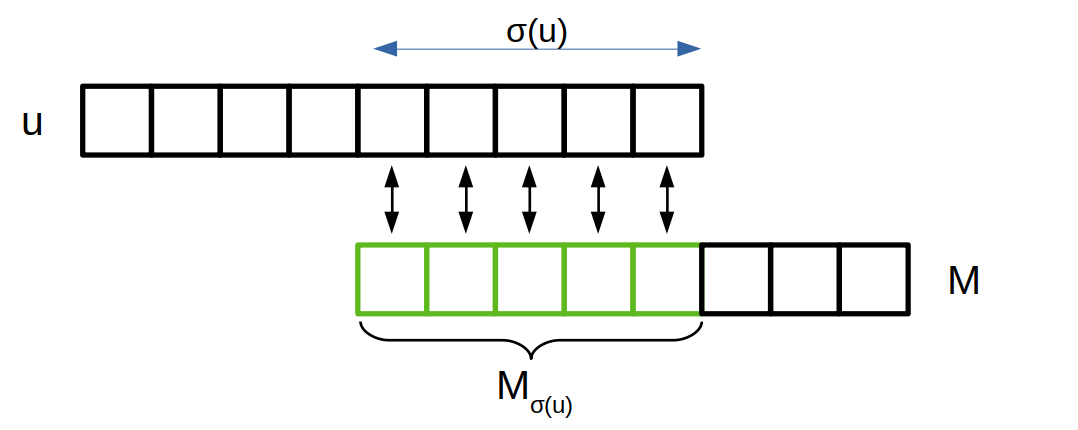
\includegraphics[scale=0.3]{nouveau_dev/Recherche de motif/cas_sans_a.png}\\ \enspace \\
		$\big\downarrow$\\ \enspace \\
		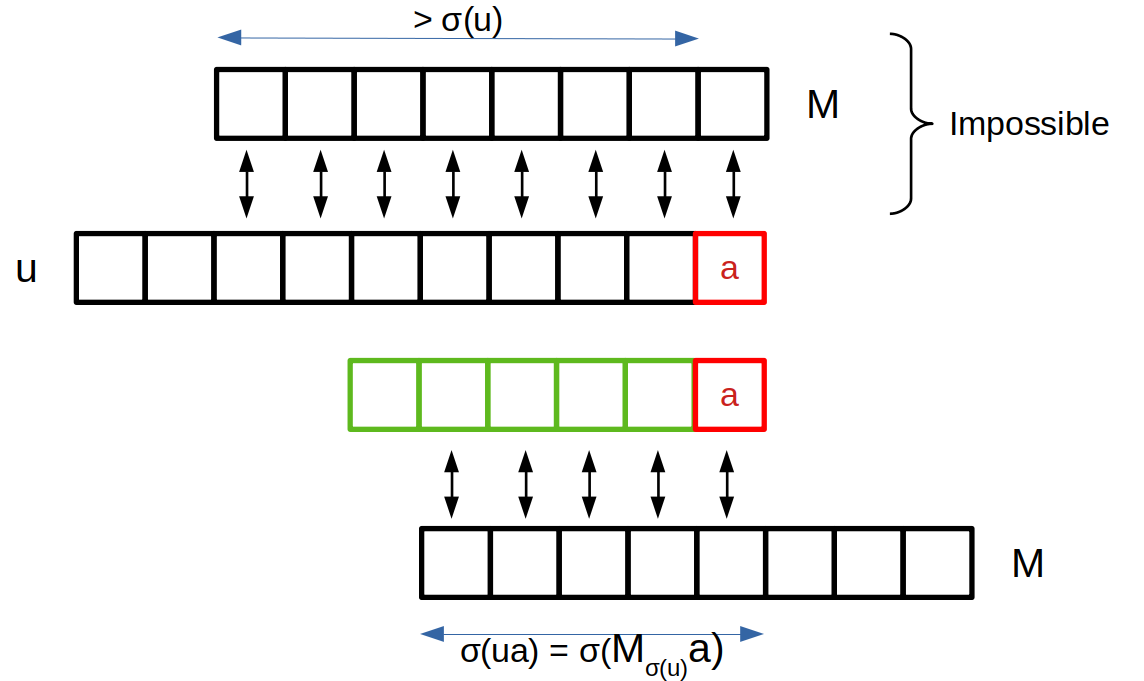
\includegraphics[scale=0.3]{nouveau_dev/Recherche de motif/cas_avec_a.png}
	\end{center}
\end{proof}
\end{itemize}
Cela conclut la récurrence.
\end{proof}

\paragraph{Conclusion} Par définition de $\sigma$, $\sigma(u)=k$ si et seulement si $M \sqsubset u$. Ainsi, 
$$
u\in \mathcal L(\mathcal A) \Leftrightarrow \delta^*(0,u)=k \Leftrightarrow \sigma(u)=k \Leftrightarrow M \sqsubset u \Leftrightarrow u \in \Sigma^*M
$$
et donc $\mathcal L(\mathcal A)=\Sigma^*M$.


\begin{proposition}
	Aucun état de $\mathcal A$ n'est inutile.
\end{proposition}

\begin{proof}
	
\begin{itemize}[label=$\bullet$]
	\item Accessibilité : $\delta^*(O, M_i) = i$ donc tous les états sont accessibles
	\item Séparabilité : Soit $0 \leq i < j \leq k$. Montrons $\exists u \: : \: \left\{\begin{array}{l}
		\delta^*(i,u) \notin F\\
		\delta^*(j,u) \in F\\
	\end{array}\right.$\\
	On note $N_i=m_{i+1}...m_k$ le suffixe de $M$ de taille $k-i$. Prenons alors $u = N_j$.\\
	$\delta^*(j, N_j) = k$\\
	et $\delta^*(i, N_j) < k$ \qquad car $|m_1\dots m_i m_{j+1} \dots m_k| < k$
\end{itemize}

\end{proof}


\paragraph{Algorithme.}

La construction de $A$ (et plus particulièrement de sa fonction de transition $\delta$) n'utilise que le motif $M$ et non le texte $T$. On peut représenter cette fonction via un tableau bidimensionnelle de taille $(k+1)\times |\Sigma|$. On peut alors remplir cette table avec les différentes valeurs de $\sigma$, ce qui se fait en temps polynomial en $k$. Enfin, on lit le texte $T$ lettre par lettre et si on atteint l'état $k$, on a trouvé une occurrence de du motif $M$. Si on atteint la fin de $T$ sans jamais atteindre $k$, alors $M$ n'apparaît pas dans $T$.
